
A key component in the object recognition pipeline is to extract robust yet representative features from perceptual inputs, usually in the format of raw pixels. Such features should be able to further support high-level interpretations such as categorization and detection, and the vision community has converged to specific architectures for feature extraction in the recent decade. Most notably, such architectures use a convolutional approach that encodes local image patches and spatially pools the output, and then stacks such convolutional components in a multi-layer fashion to build mid and high level features. Despite various ways on how such networks should be constructed (e.g.\ with handcrafted features or fully trained), such structures have remained effective in various applications, including digit recognition \cite{lecun1998gradient}, object detection \cite{Dalal:2005to}, object classification \cite{Yang:2009vb}, and the recent success of convolutional neural networks in large-scale classification tasks \cite{krizhevsky2012imagenet}.

This chapter focuses on the building block of such approaches - a single-layer network that contain one local coding stage and one spatial pooling stage. Specifically, we proposes a novel approach to perform pooling to obtain more selective features for object recognition, achieving higher performance on benchmark datasets than conventional pooling approaches do. We then explain the theoretical justification of a common phenomenon found in the single-layer network analysis: higher dimensional features almost always lead to better classification performance. This chapter focuses on the single-layer network for clarity, but the results we found would apply to multi-layer networks as well.

\section{Background}

Overcompletely encoded features have been shown to provide state-of-the-art performance on various applications. In computer vision, locally encoded and spatially pooled feature extraction pipelines work particularly well for image classification. Such pipelines usually start from densely extracted local image patches (either normalized raw pixel values or hand-crafted descriptors such as SIFT or HOG), and perform dictionary learning to obtain a dictionary of codes (also called filters). The patches are then encoded into an over-complete representation using various algorithms such as sparse coding \cite{Olshausen:1997uh,wang2010locality} or simple inner product with a non-linear post-processing \cite{coates2011icml,krizhevsky2012imagenet}. After encoding, spatial pooling with average or max operations are carried out to form a global image representation \cite{Yang:2009vb,Boureau:uq}. The encoding and pooling pipeline may be stacked in a deep structure to produce a final feature vector, which is then used to predict the labels for the images usually via a linear classifier or a densely connected multilayer neural network.

During the last decade, much emphasis has been directed at the coding step. Dictionary learning algorithms have been discussed to find a set of basis that reconstructs local image patches or descriptors well \cite{mairal2010online,coates2011icml}, and several encoding methods have been proposed to map the original data to a high-dimensional space that emphasizes certain properties, such as sparsity \cite{Olshausen:1997uh,Yang:2009vb,yang2010efficient} or locality \cite{wang2010locality}. Recent papers \cite{coates2010aistats, Rigamonti:2011uc, coates2011icml} have explored the relationship between dictionary learning and encoding, and have proposed simple yet effective approaches that achieve competitive results. The neuroscience justification of coding comes from simple neurons in the human visual cortex V1, which have been believed to produce sparse and overcomplete activations \cite{Olshausen:1997uh}.

Similarly, the idea of spatial pooling dates back to Hubel's seminal paper about complex cells in the mammalian visual cortex \cite{Hubel:1962vm}, which identifies mid-level image features that are invariant to small spatial shifting. The spatial invariance property also reflects the concept of locally orderless images \cite{Koenderink:1999bh}, which suggests that low-level features are grouped spatially to provide information about the overall semantics. Most recent research on spatial pooling aims to find a good pooling operator, which could be seen as a function that produces informative statistics based on local features in a specific spatial area. For example, average and max pooling strategies have been found in various algorithms respectively, and systematic comparisons between such pooling strategies have been presented and discussed in \cite{Boureau:uq,Boureau:2010wz}. Recently, Coates et al.\ proposed to pool over multiple features in the context of deep learning \cite{coates2011selecting}.

However, relatively little effort has been put into better designs or learning of better spatial regions for pooling, although it has been discussed in the context of learning local descriptors \cite{winder2007learning}. A predominant approach to define the spatial regions for pooling, which we will also call the receptive fields (borrowing the terminology from neuroscience) for the pooled features, comes from the idea of spatial pyramids \cite{lazebnik2006beyond, Yang:2009vb}, where regular grids of increasing granularity are used to pool local features. The spatial pyramids provide a reasonable cover over the image space with scale information, and most existing classification methods either use them directly, or use slightly modified/simplified versions.

In addition, recent research has revealed a particularly interesting finding \cite{coates2010aistats, Rigamonti:2011uc, coates2011icml, saxe2011random} that very simple patch-based algorithms like K-means or even random selection, combined with feed-forward encoding methods with a naive nonlinearity, produces state-of-the-art performance on various datasets. Explanation of such phenomenon often focuses on the local image patch statistics, such as the frequency selectivity of random samples \cite{saxe2011random}, but does not offer an asymptotic theory on the dictionary learning behavior. We will show later in the chapter that a \nystrom sampling based interpretation explains such phenomenon well by providing asymptotic bounds to the observed accuracy, and that such interpretation will lead to an efficient, unsupervised feature selection paradigm.

\section{The Classification Pipeline}\label{sec:pipeline}

\begin{figure*}[t]
  \centering
  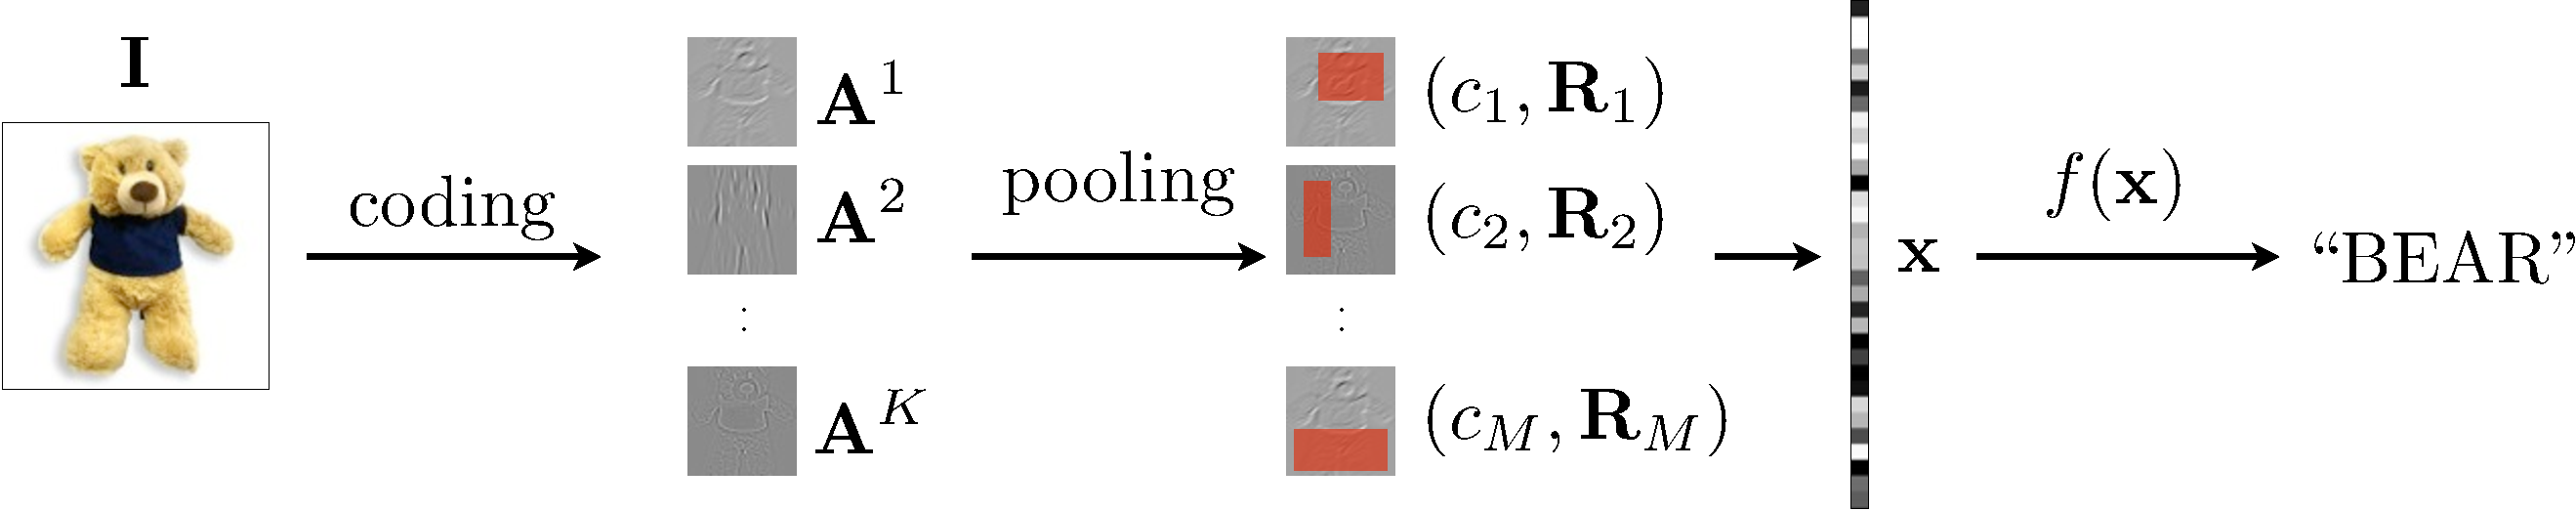
\includegraphics[width=1.\textwidth]{figs/smartpooling/pipeline_cvpr.pdf}
  \caption{The image classification pipeline. See Section \ref{sec:pipeline} for details.}\label{fig:pipeline}
  \vspace{-0.15in}
\end{figure*}

Before the introduction of the proposed methods, we briefly review the image classification pipeline we adopted, which leads to the problem of learning the receptive fields for spatial pooling. Specifically, we will focus on two-layer classification approaches.

We illustrate the pipeline from raw images to the prediction of class labels in Figure \ref{fig:pipeline}. Specifically, starting with an input image $\bI$, two stages are usually adopted to generate the global feature, as we formally define below.

\paragraph{(1) Coding.} In the coding step, we extract local image patches, and encode each patch to $K$ activation values based on a codebook of size $K$ (learned via a separate dictionary learning step). These activations are typically binary (in the case of vector quantization) or continuous (in the case of e.g.\ sparse coding). It is generally believed that having an overcomplete ($K \gg$ the dimension of patches) codebook while keeping the activations sparse helps classification, especially when linear classifiers are used in the later steps.

Recently, Coates et al.~\cite{coates2011icml} have shown that relatively simple dictionary learning and encoding approaches lead to surprisingly good performances. To learn a dictionary $\bD =[\bd_1,\bd_2,\cdots,\bd_K]$ of size $K$ from randomly sampled patches $\{\bp_1,\bp_2,\cdots,\bp_N\}$ each reshaped as a vector of pixel values, two simple yet effective approaches are advocated:
\begin{enumerate}
  \item K-means, which minimizes the squared distance between each patch and its nearest code: $\min_{\bD} \sum_{i=1}^{N}\min_{j}\|\bp_i - \bd_j\|_2^2$.
  \item OMP-M, which learns a dictionary that minimizes the reconstruction error, with the constraint that each patch is modeled by a linear combination of at most $M$ codes: $\min_{\bD,\balpha_{i}} \sum_{i=1}^{N}\|\bp_i-\bD\balpha_i\|^{2}_{2}$, where the length of each dictionary entry $\bd_j$ is $1$, and the cardinality of each reconstruction coefficient $\balpha_i$ is at most $M$.
\end{enumerate}
For encoding, Coates et al.\ also propose to substitute sparse coding by the following efficient approaches:
\begin{enumerate}
  \item Triangle coding \cite{coates2010aistats}, which computes the activation of code $k$ for a patch $\bp$ as $f_k(\bx) = \max\{0,\mu(\bz) - z_k\}$, where $z_k$ is the distance from $\bp$ to the $k$-th code $\bd_k$, and $\mu(\bz)$ is the mean of distances from $\bp$ to all codes. 
  \item Soft thresholding, which computes the inner product between $\bp$ and each code, with a fixed threshold parameter $\alpha$: $f_{k}(\bx) = \max\{0, \bd_k^\top\bp - \alpha\}$
\end{enumerate}

We refer to \cite{coates2011icml} for a systematic discussion about different dictionary learning and encoding algorithms. In our experiment, we will adopt these standard approaches in order to isolate  the contribution of spatial pooling from the choice of different coding methods. Since local patches are usually extracted densely in a grid-based fashion, we will organize the activations of image $\bI$ as a set of matrices denoted by $\{\bA^{1}(\bI)\bA^{2}(\bI),\cdots,\bA^{K}(\bI)\}$, one for each code in the codebook, whose element $A_{ij}^k(\bI)$ contains the activation of code $\bd_k$ for the local image patch at spatial location $(i,j)$. 

\paragraph{(2) Pooling.} Since the coding result are highly overcomplete and highly redundant, the pooling layer aggregates the activations over certain spatial regions of the image to obtain an $M$ dimensional vector $\bx$ as the global representation of the image. Each dimension of the pooled feature $\bx_i$ is obtained by taking the activations of one code in a specific spatial region (shown as the red rectangular in Figure \ref{fig:pipeline}), and performing a predefined operator (usually average or max) on the set of activations. 

We follow a similar approach to that in \cite{Boureau:2011tz} to formally define pooled features. Specifically, given an operator $\operatorname{op}$ that maps a set of real values to a single real value (e.g.\ by taking their average), a pooled feature $x_i$ can be defined based on the selection of a code indexed by $c_i$ and a spatial region denoted by $\bR_{i}$:
\begin{equation}
  x_i = \operatorname{op} (\bA^{c_i}_{\bR_{i}})
\end{equation}
Borrowing the definition from neuroscience, we call $\bR_i$ the \emph{receptive field} for the pooled feature, which could be seen as a binary mask over the image. $\bA^{c_i}_{\bR_{i}}$ is then the set of activations of code $c_i$ in the receptive field $\bR_i$.

This definition provides a general definition that embraces existing pooling algorithms. For example, commonly used operators involve computing the statistics of the activations under the $p$-norm:
\begin{equation}
  x_i = \frac{1}{|\bR_{i}|}(\sum\nolimits_{\alpha_i \in \bA^{c_i}_{\bR_{i}}} \alpha_i^{p})^{\frac{1}{p}}
\end{equation}
when $p=1$ this corresponds to the average pooling, and when $p\rightarrow \infty$ this corresponds to the max pooling.

We focus on the definition of receptive fields for pooling. The simplest form of pooling takes the whole image as the receptive field, thus assuming a bag-of-words model where spatial information is ignored. The more commonly adopted spatial pooling approach \cite{lazebnik2006beyond,Yang:2009vb} pools features from multiple levels of regular grids, thus defining a pyramid of pooled features. Given a set of $K$ codes and a set of $N$ receptive fields, the pooled features are then defined by taking the Cartesian product of the codes and the receptive fields, yielding a $KN$-dimenisonal global feature.

Finally, a classifier, usually linear SVM or logistic regression, is trained using the global feature vector to predict the final label of the image as $y = f(\bx;\btheta)$.

\section{Receptive Field Learning for Pooled Image Features}\label{sec:grafting}
While significant efforts have been placed on the coding part of the classification pipeline, the pooling step has received relatively little attention. Existing research on pooling mainly focuses on the analysis of the pooling operator, such as in \cite{Boureau:2010wz}. Specifically, spatial regions are almost always defined on regular grids \cite{Yang:2009vb}, which may not guarantee to be optimal. As a simple example, to distinguish most indoor and outdoor scenes, a human may look for the existence of the horizon, which could be captured by thin horizontal pooling regions over the image. Spatial grids, even with a pyramid structure, fail to provide such information. Such receptive fields may be dataset-dependent, leading us to ask the question \emph{``are spatial pyramids optimal for image classification?''}, the answer to which is often neglected by existing algorithms.

Instead of arbitrarily defining heuristic receptive fields, we aim to explicitly learn the receptive fields for classification tasks. Specifically, we propose to adaptively learn such regions by considering the receptive fields additional parameters, and jointly learning these parameters with the subsequent classifiers. The resulting benefit is two-fold: receptive fields tailored to classification tasks increase the overall accuracy of classification; in addition, with the help of such mid-level features, we are able to use a much lower-dimensional feature to achieve the state-of-the-art performance. We experiment with our algorithm on the benchmark CIFAR-10 dataset and other datasets, and report a significant improvement in both accuracy and efficiency.

Inspired by the selectivity of complex cells in the visual cortex, we propose to learn the pooled features adaptively. Specifically, learning a set of $M$ pooled features is equivalent to learning the parameters $\mathcal{C} = \{c_1,c_2,\cdots,c_M\}$ and $\mathcal{R} = \{\bR_1,\bR_2,\cdots,\bR_M\}$ \footnote{For simplicity, we will use the $\max$ operator, but note that any operator could also be incorporated in our framework.}. To this end, we note that the pooled features are directly fed into the final classifier, and propose to jointly learn the classifier parameters $\btheta$ together with the pooling parameters. Thus, given a set of training data $\mathcal{X} = \{(\bI_n,\by_n)\}_{n=1}^{N}$, the joint learning leads to solving the following optimization problem:
\begin{eqnarray}\label{eqn:adaptiverecfield}
  \min_{\mathcal{C},\mathcal{R},\btheta} & & \frac{1}{N}\sum_{n=1}^{N}\mathcal{L}(f(\bx_n;\btheta),\by_n) + \lambda\operatorname{Reg}(\btheta)\\
  \text{where} & & x_{ni} = \operatorname{op} (\bA^{c_i}_{n,\bR_{i}})\nonumber
\end{eqnarray}
where we assume that the coding from $\bI_{n}$ to $\{\bA^{c_i}_{n}\}_{i=1}^{K}$ is done in an unsupervised fashion, as has been suggested by several papers such as \cite{coates2010aistats}. We call this method receptive field learning, as the receptive fields are learned in such a way that information most relevant to the classification task will be extracted.

One practical issue is that solving the optimization problem (\ref{eqn:adaptiverecfield}) may be impractical, as there is an exponential number of receptive field candidates, leading to a combinatorial problem. Numerical solutions are also difficult, as the gradient with respect to the pooling parameters is not well-defined. Thus, instead of searching in the space of all possible receptive fields, we adopt the idea of over-completeness in the sparse coding community. Specifically, we start from a set of reasonably overcomplete set of potential receptive fields, and then find a sparse subset of such pooled features. The over-completeness enables us to maintain performance, while the sparsity allows us to still carry out classification efficiently during testing time.

\begin{figure}
  \centering
  \begin{tabular}{ccc}
    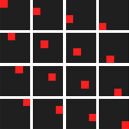
\includegraphics[width=0.27\linewidth]{figs/smartpooling/basebins.png} & %
    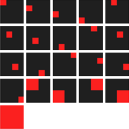
\includegraphics[width=0.27\linewidth]{figs/smartpooling/spmbins.png} & %
    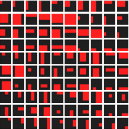
\includegraphics[width=0.27\linewidth]{figs/smartpooling/ocbins.png}\\
    (a) & (b) & (c)
  \end{tabular}
  \caption{An example of overcomplete rectangular bins based on a $4\times 4$ superpixel setting: (a) superpixels; (b) spatial pyramid bins; (c) overcomplete rectangular bins.}\label{fig:ocbins} 
\end{figure}

\subsection{Overcomplete Receptive Fields}
The exponential number of possible receptive fields arises when we consider the inclusion and exclusion of single pixels individually. In practice this is often unnecessary, as we expect the active pixels in a receptive field to be spatially contiguous. In this paper, we use receptive fields consisting of rectangular regions\footnote{As a side note, we also experimented with receptive fields that are sampled from an Ising model on the fly during training, but rectangular regions worked empirically better, possibly because the additional flexibility of Ising models leads to over-fitting the training data, and the spatial inconsistency may render randomly sampled receptive fields not as useful in classification tasks.}: this provides us a reasonable level of over-completeness, as there are $O(n^4)$ different rectangular receptive fields for an image containing $n\times n$ pixels. In addition, since the motivation of spatial pooling is to provide tolerance to small spatial displacements, we build the rectangular regions upon superpixels, which are defined as dense regular grids on the image. Figure \ref{fig:ocbins} shows an example of such rectangular receptive fields compared with regions defined by the spatial pyramid on a $4\times4$ grid.

Given the set of $P$ overcomplete regions, which we denote by $\mathcal{R} = \{\bR_{1},\bR_{2},\cdots,\bR_{P}\}$, and the dictionary $\mathcal{D} = \{\bd_1,\bd_2,\cdots,\bd_K\}$ of size $K$, we can define a set of $PK$ potential pooled features based the Cartesian product $\mathcal{R}\times\mathcal{D}$. Specifically, the $i$-th receptive field and the $j$-th code jointly defines the $(K\times i + j)$-th pooled feature as $x_{K\times i + j} = \operatorname{op} (\bA_{\bR_i}^{j})$. Note that when the coding and pooling are both carried out in an overcomplete fashion, the resulting pooled feature is usually very high-dimensional.

\subsection{Structured Sparsity for Receptive Field Learning}
While it is possible to train a linear classifier using the high-dimensional pooled feature $\bx$ above, in practice it is usually beneficial to build a classifier using relatively low-dimensional features. In addition, for multiple-label classification, we want the classifiers of different labels to share features. This brings two potential advantages: feature computation could be minimized, and sharing features among different classifiers is known to provide robustness to the learned classifiers. To this end, we adopt the idea of structured sparsity \cite{quattoni2008transfer,schmidt2008structure}, and train a multiple-class linear classifier $\by = f(\bx) = \bW\bx + \bb$ via the following optimization problem:
\begin{equation}\label{eqn:structuredsparsity}
  \min_{\bW,\bb} \quad \frac{1}{N}\sum_{n=1}^{N}l(\bW^\top\bx_n+\bb, \by_n) + \frac{\lambda_1}{1}\|\bW\|_{\mathrm{Fro}}^{2} + \lambda_2\|\bW\|_{1,\infty}
\end{equation}
where $\by_i$ is the $L$-dimensional label vector coded in a $1-of-L$ fashion, with values taken from $\{-1,+1\}$ given $L$ classes. $\bx_i$ is an $M$-dimensional feature vector defined by overcomplete pooling in the previous subsection, and $\bW = [\bw_1,\bw_2,\cdots, \bw_L]$ is a $M\times L$ weight matrix containing the weight vector for the $L$ classifiers. 

Two regularization terms are adopted in the optimization. The squared Frobenius norm $\|\bW\|_{\mathrm{Fro}}^2$ aims to minimize the structured loss in the classical SVM fashion, and the second regularizer is the $L_{1,\infty}$ norm of the matrix $\bW$:
\begin{equation}
  \|\bW\|_{1,\infty} = \sum_{i=1}^{M} \|\bW_{i,\cdot}\|_{\infty} = \sum_{i=1}^{M}\max_{j\in\{1,\cdots,L\}} |W_{ij}|
\end{equation}
where $\bW_{i,\cdot}$ denotes the $i$-th row of the matrix $W$. This regularizer introduces structured sparsity by encouraging the weight matrix $\bW$ to be row-wise sparse, so that the classifiers for different classes tend to agree on whether to use a specific feature, and when combined together, only jointly use a subset of the overcomplete pooled features. The addition of the $L_{1,\infty}$ norm also provides a elastic-net like regularization, which is known to perform well when the dimension of data is much higher than the number of data points \cite{zou2005regularization}.

For optimization considerations, we use the multi-class extension of the binomial negative log likelihood (BNLL) loss function \cite{Perkins:2003vc}:
\begin{equation}
  l(\bW^\top\bx + \bb, \by) = \sum_{i=1}^{L}\ln(1+e^{-\by_i(\bW_{\cdot,i}^\top \bx + b_i)})
\end{equation}
The choice of the BNLL loss function over the hinge loss is mainly for computational simplicity, as the gradient is easier to compute for any input. In practice, the performance does not change much if we use the hinge loss instead.

\section{Fast Approximate Learning with Feature Grafting}
Jointly optimizing (\ref{eqn:structuredsparsity}) is still a computationally challenging task despite its convexity, due to the over-completeness in both coding and pooling. While it is possible to carry out the computation on smaller-scale problems like Caltech-101, we adopt a greedy approach to train the model for larger-scale problems. Inspired by the matching pursuit algorithm in dictionary training and the grafting algorithm \cite{Perkins:2003vc} in machine learning, we start with an empty set of selected features, incrementally add features to the set, and retrain the model when new features are added. 

\begin{figure}
  \centering
  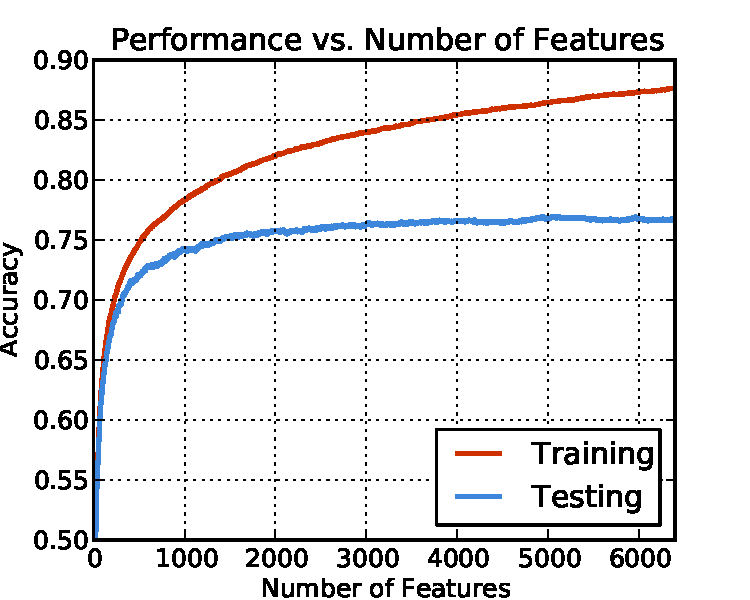
\includegraphics[width=0.5\textwidth]{figs/smartpooling/grafting_perf.pdf}
  \caption{Performance vs.\ number of selected features, with the experiment setting in Table \ref{table:gridsize} of Section \ref{sec:experiments}.}\label{fig:graftingsteps}
\end{figure}

Mathematically, we maintain a set $\mathcal{S}$ recording the set of currently selected features. At each iteration, for each feature index $j$ that has not been not selected, we compute the score of the feature as the 2-norm of the gradient of the objective function (\ref{eqn:structuredsparsity}), denoted by $\Loss(\bW,\bb)$, with respect to the corresponding weight vectors:
\begin{eqnarray}
  \operatorname{score}(j) = \left\|\frac{\partial \Loss(\bW,\bb)}{\partial \bW_{j,\cdot}}\right\|_\mathrm{Fro}^2
\end{eqnarray}

We then select the feature with the largest score, and add it to the selected set $\mathcal{S}$. The model is retrained using the previously learned optimum solution as the starting point. From a boosting perspective, this can be considered as incrementally learning weak classifiers, but our method differs from boosting in the sense that the weights for already selected features are also updated when new features are selected.

As the speed of retraining drops when more features are added, we adopt an approximate retraining strategy: for each iteration $t$, we select an active subset $\mathcal{S}_{A}$ of $\mathcal{S}$ based on the score above. We then retrain the model with respect to the active set and the bias term only:
\begin{equation}
  \bW^{(t+1)}_{\mathcal{S}_A,\cdot}, \bb = \operatorname{\arg\min}_{\bW_{\mathcal{S}_A,\cdot},\bb}\Loss(\bW,\bb)
\end{equation}
with the constraint that $\bW_{\bar{\mathcal{S}_A},\cdot}$ keep unchanged. The intuition is that with an already trained classifier from the previous iteration, adding one dimension will only introduce small changes to the existing weights. 

In practice, we found the performance of this approximate algorithm with the active set size less than 100 to be very close to the full retraining algorithm with a significant increase in computation speed. Figure \ref{fig:graftingsteps} shows typical curves of the training and testing accuracy with respect to the number of iterations. The performance usually stabilizes with a significantly smaller number of features, showing the effectiveness of introducing structured sparsity into classifier learning.

\section{Experiments}\label{sec:experiments}
We will mainly report the performance of our algorithm on the CIFAR-10 dataset\footnote{http://www.cs.toronto.edu/~kriz/cifar.html}, which contains 50,000 $32\times32$ images from 10 categories as training data, and 10,000 images as testing data.

We fix the dictionary learning algorithms to k-means clustering and the coding algorithms to triangular coding as proposed in \cite{coates2010aistats} for CFAR-10. Such a coding strategy has been shown to be particularly effective in spite of its simplicity. We also tested alternative dictionary learning and coding algorithms, which led to similar conclusions. As our main focus is on learning receptive fields for pooled features, the results of different coding algorithms are omitted, and we refer to \cite{coates2011icml} for a detailed discussion about dictionary learning and coding algorithms. 

For classification, when we use pre-defined receptive fields such as spatial pyramids, the SVM regularization term is chosen via 5-fold cross validation on the training data. When we perform feature selection, we fix $\lambda_1 = 0.01$ (which is the best value when performing 5-fold cross validation for max pooling on a 2$\times$2 regular grid) and drop $\lambda_2$, since the incremental feature selection already serves as a greedy approximation of the sparse constraint. Although the parameters are not tuned specifically for each configuration, we found it to perform well empirically under various scenarios.

\subsection{Spatial Pyramid Revisited}
It is interesting to empirically evaluate the performance of spatial pyramid regions against other choices of receptive fields. To this end, we trained a dictionary of size 200 (for speed considerations), and tested the performance of 3-layer spatial pyramid pooling against two algorithms based on overcomplete receptive fields: (1) random selection from the overcomplete pooled features, and (2) our method, both selecting the same number of features that spatial pyramid pooling uses. Results are shown in Figure \ref{fig:spmvsrandomvsgraft}. Our method outperforms SPM, but a more interesting finding is that the predefined spatial pyramid regions perform consistently worse than random selection, indicating that arbitrarily defined pooled features may not capture the statistics of real-world data well. With explicit learning of the pooling parameters, we achieved the highest performance among the three algorithms, showing the effectiveness and necessity of learning adaptive receptive fields.

\begin{figure}
  \centering
  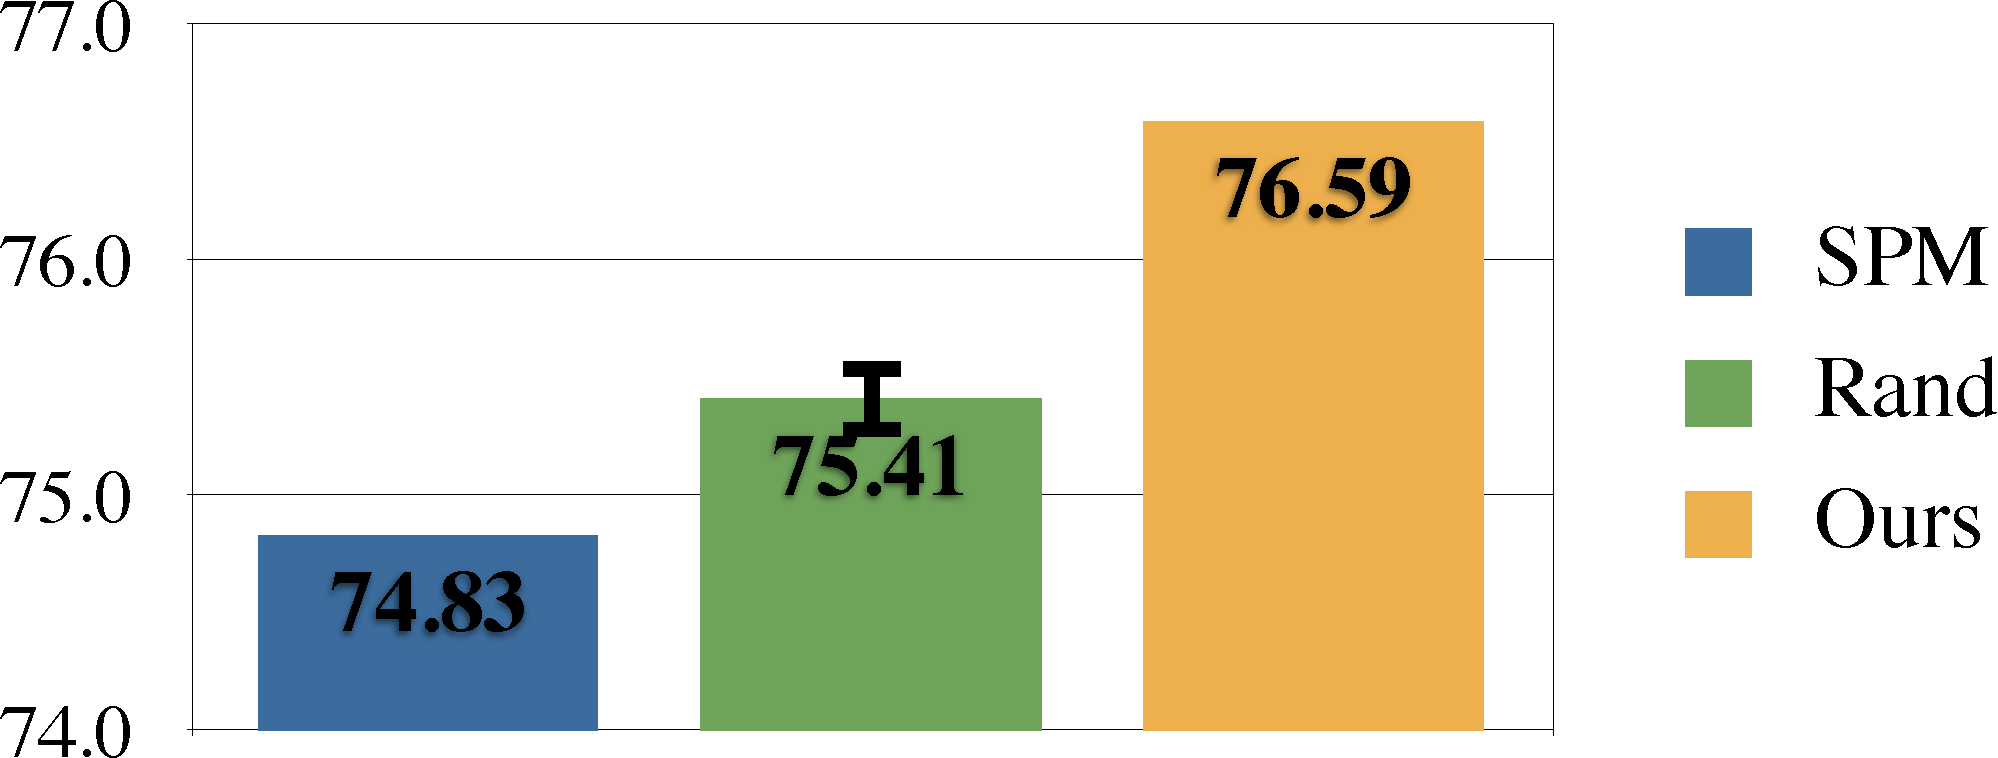
\includegraphics[width=0.5\textwidth]{figs/smartpooling/perfcomparison.pdf}
  \caption{Performance comparison among spatial pyramid pooling, random feature selection and our method, all using the same number of features for the final classification. It can be observed that a few selected features could already achieve a comparatively high performance.}\label{fig:spmvsrandomvsgraft}
\end{figure}

\subsection{The Effect of Spatial Over-completeness}

One may ask if the performance increase could be obtained without overcompletenes by simply using a denser grid. To answer this question, we examined the performance of our algorithm against the 2$\times$2 pooling grid (which is used in \cite{coates2011icml} to obtain very high performance) and a denser $4\times4$ grid, with both average and max poolings. We also compared our method against random feature selection from the same pooling candidates. Table \ref{table:gridsize} summarizes the testing accuracy under various experimental settings, using a codebook size of 200.

Results from Table \ref{table:gridsize} demonstrates that denser pooling does help performance. The 4$\times$4 grid increases the performance by about 3 percent compared to 2$\times$2 pooling. However, with overcomplete receptive fields we can almost always increase performance further. We achieved an 76.72\% accuracy with only 200 codes, already close with state-of-the-art algorithms using much larger codebook sizes (Table \ref{table:cifar10}). It is also worth pointing out that even random feature selection gives us comparable or better performance when compared to pre-defined pooling grids under the same number of feature dimension (e.g.\ compare the performance between $4\times4$ max pooling and randomly selecting $3,200$ features from an overcomplete set of pooled features). 

Further, the importance of feature selection lies in two aspects: first, simply using all the features is not practical during testing time, as the dimension can easily go to hundreds of thousands when we increase the codebook size. Feature selection is able to get very close performance compared to using all the features, but with a significantly lower dimensionality, which is essential in many practical scenarios. Usually, feature selection enables us to achieve a high performance with only a few features (Figure \ref{fig:graftingsteps}). Adding remaining features will only contribute negligibly to the overall performance. Second, performing feature selection has the potential benefit of removing redundancy, thus increasing the generalization ability of the learned classifiers \cite{Perkins:2003vc,tibshirani1996regression}. In our experiment in Table \ref{table:gridsize}, the best performance is achieved with a few thousands features. Similarly, we found that with larger codebook sizes, using all the overcomplete pooled features actually decreases performance, arguably due to the decrease of the generalization ability. 

% Notes: In case you are wondering, these numbers are obtained using the same codebook. It is run on the NEC skyservers, and the codebook is stored in the git repository logs/codebooks/200.mat.
\begin{table}
  \centering
  \begin{tabular}{r|r|r|c}
    \hline
    Pooling Area & Method & Features & Accuracy\\
    \hline
    2$\times$2 & Ave & 800 & 70.24\\
    4$\times$4 & Ave & 3,200 & 72.24\\
    2$\times$2 & Max & 800 & 66.31\\
    4$\times$4 & Max & 3,200 & 73.03\\
    3-layer SPM & Max & 4,200 & 74.83\\ % training 82.54%
    \hline
    OC + feat select & Max & 800 & 73.42\\
                  &     & 3,200 & 76.28\\
                  &     & 4,200 & 76.59\\
                  &     & 6,400 & {\bfseries 76.72}\\
    \hline
    OC, all features & Max & 20,000 & 76.44\\ % training 0.91064
    OC + rand select & Max & 800 & 69.48\\ % standard deviation 0.3442
    OC + rand select & Max & 3,200 & 74.42\\ % standard deviation 0.21247
    OC + rand select & Max & 4,200 & 75.41\\ % standard deviation 0.159
    \hline
  \end{tabular}
  \caption{Comparison of different pre-defined pooling strategies and our method (overcomplete (OC) + feature selection). Random selection from the same overcomplete pooled features is also listed, showing the necessity of better receptive field learning.}\label{table:gridsize}
\end{table}

\subsection{Larger Codebook vs.\ Better Spatial Pooling}
Under the two-stage pipeline adopted in this paper, there are effectively two possible directions to increase the performance: to increase the codebook size and to increase the pooling over-completeness. We argue that these two directions are complementary: the performance gain from our effort on pooling could not simply be replaced by increasing the codebook size, at least not easily. More importantly, as the codebook size grows larger, it becomes more difficult to obtain further performance gain, while it is still relatively easy to obtain gains from better pooling.

To empirically justify this argument, we trained multiple codebooks of different sizes, and compared the resulting accuracies with and without overcomplete pooling in Figure \ref{fig:ocpooling}. As can be observed, it becomes harder to obtain further performance gain by increasing the codebook size when we already have a large codebook, while using a better pooling strategy always brings additional accuracy gains. In fact, with our method, we are able to use a codebook of half the size (and half the number of pooled features) while maintaining performance (compare the green and blue curves). It is particularly interesting that, by selecting more features from the overcomplete spatial regions, we are able to achieve state-of-the-art performance with a much smaller number of codes (the red curve), which has the potential in time-sensitive or memory-bounded scenarios.

\begin{figure}
  \centering
  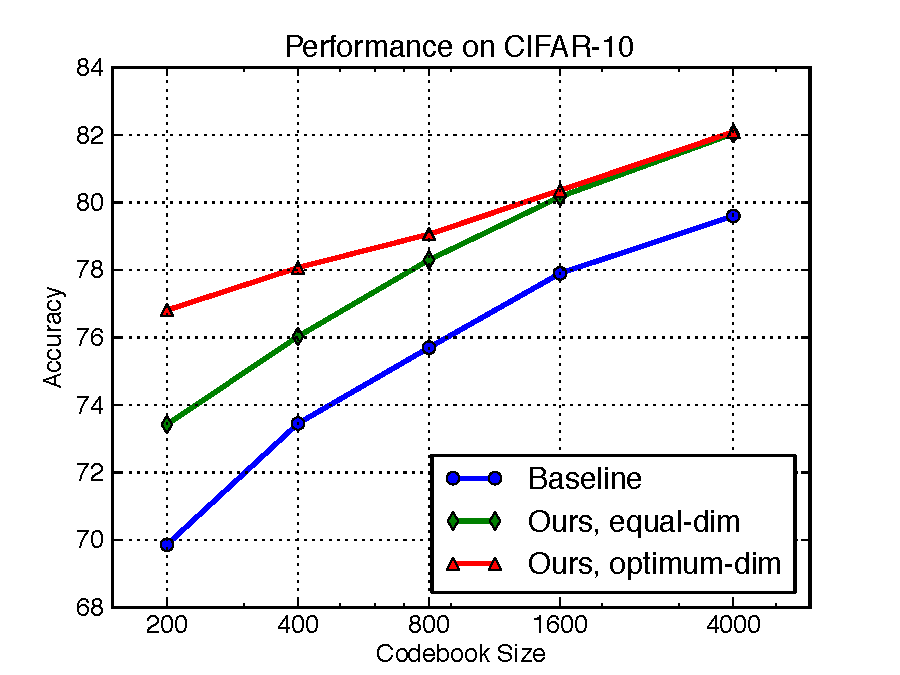
\includegraphics[width=0.5\textwidth]{figs/smartpooling/perf_vs_codes.pdf}
  \caption{Testing accuracies on CIFAR-10 with and without overcomplete pooling. In the figure, ``equal-dim'' selects the same number of features as the baseline (Coates et al.\cite{coates2010aistats}), and ``optimum-dim'' selects the optimum number of features determined by cross-validation. (X-axis in log scale)}
  \label{fig:ocpooling}
\end{figure}

\begin{table}
  \begin{minipage}[c]{1\linewidth}
  \begin{center}
  \begin{tabular}{c|r|c}
    \hline
    Method & Pooled Features & Accuracy \\
    \hline
    ours, d=1600 & 6,400 & 80.17 \\
    ours, d=4000 & 16,000 & 82.04 \\
    ours, d=6000 & 24,000 & {\bfseries 83.11}\\
    \hline
    Coates et al. \cite{coates2010aistats}, d=1600 & 6,400 & 77.9\phantom{0} \\
    Coates et al. \cite{coates2010aistats}, d=4000 & 16,000 & 79.6\phantom{0} \\
    Coates et al. \cite{coates2011icml}, d=6000 & 48,000 & 81.5\phantom{0}\\
    \hline
    Conv. DBN \cite{Krizhevsky2010} & N/A & 78.9\phantom{0} \\
    Improved LCC \cite{Yu:2010wu} & N/A & 74.5\phantom{0} \\
    8-layer Deep NN \cite{2011arXiv1102.0183C} & N/A & 80.49 \\
    3-layer Deep NN \cite{coates2011selecting} & N/A & 82.0\phantom{0} \\
    \hline
  \end{tabular}
  \end{center}
  \end{minipage}
  \caption{Performance on the CIFAR-10 dataset. The first and second blocks compare performance between our method and Coates et al. \cite{coates2010aistats,coates2011icml} under similar codebook sizes, where the only difference is the spatial pooling strategy. The third block reports the performance of several state-of-the-art methods in the literature.}\label{table:cifar10}
\end{table}

\subsection{Best Performance}
Our best performance on the CIFAR-10 dataset was achieved by training a codebook size of 6,000, performing max pooling on overcomplete rectangular bins based on a $4\times4$ grid, and selecting features up to 24,000 dimensions. We also note that the accuracy has not saturated at this number of features, but we would like to test the performance when the number of mid-level features is limited to a reasonable scale. With these settings, we achieved an accuracy of 83.11\% on the testing data. To the best of our knowledge, this is the best published result on CIFAR-10 without increasing the training set size by morphing the images. 

Table \ref{table:cifar10} lists the performance of several state-of-the-art methods. It is also worth pointing out that, to achieve the same performance, our algorithm usually uses a much lower number of features compared with other well-performing algorithms.

\subsection{Results on MNIST}
We can view the set of learned receptive fields for pooling as a saliency map for classification \cite{Itti:2001wa}. To visually show the saliency map and verify its empirical correctness, we applied our method to handwritten digit recognition on the MNIST dataset, on which convolutional deep learning models are particularly effective. To this end, we adopted a similar pipeline as we did for CIFAR-10: dense 6x6 local patches with ZCA whitening are used; a dictionary of size $800$ is trained with OMP-1, and thresholding coding with $\alpha=0.25$ (untuned) is adopted. The features are then max-pooled on overcomplete rectangular areas based on a $6\times 6$ regular grid. Note that we used a different coding method from the CIFAR-10 experiment to show that the overcomplete spatial pooling method is agnostic of the choice of low-level coding algorithms. Any parameter involved in the pipeline such as SVM regularization weights is tuned on a random 50k/10k split of the training data.

Figure \ref{fig:mnist} shows the 1-vs-1 saliency maps between digits. It can be seen that by learning receptive fields, the classifier focuses on regions where the digits have maximal dissimilarity, e.g., the bottom part for 8 and 9, and the top part for 3 and 5, which matches our intuition about their appearances. For 10-digit classification, we achieved an error rate of $0.64\%$, on par with several state-of-the-art algorithms (Figure \ref{fig:mnist} left). A gap still exists between our method and the best deep-learning algorithm, and combining receptive learning with deeper structures is future work.

\begin{figure}
  \centering
  \begin{minipage}[h]{0.4\linewidth}
  \centering
  \begin{tabular}{c|c}
    \hline
    Method & err\%\\
    \hline
    Baseline \cite{coates2011icml}\footnote{Our implementation.} & 1.02\\
    {\bfseries Our Method} & {\bfseries 0.64}\\
    \hline
    Lauer et al. \cite{lauer2007trainable} & 0.83\\
    Labusch et al. \cite{labusch2008simple} & 0.59\\
    Ranzato et al. \cite{ranzato2007unsupervised} & 0.62\\
    Jarrett et al. \cite{jarrett2009best} & 0.53\\
    \hline
  \end{tabular}
  \end{minipage}\hspace{0.5in}%
  \begin{minipage}[h]{0.4\linewidth}
  \centering
  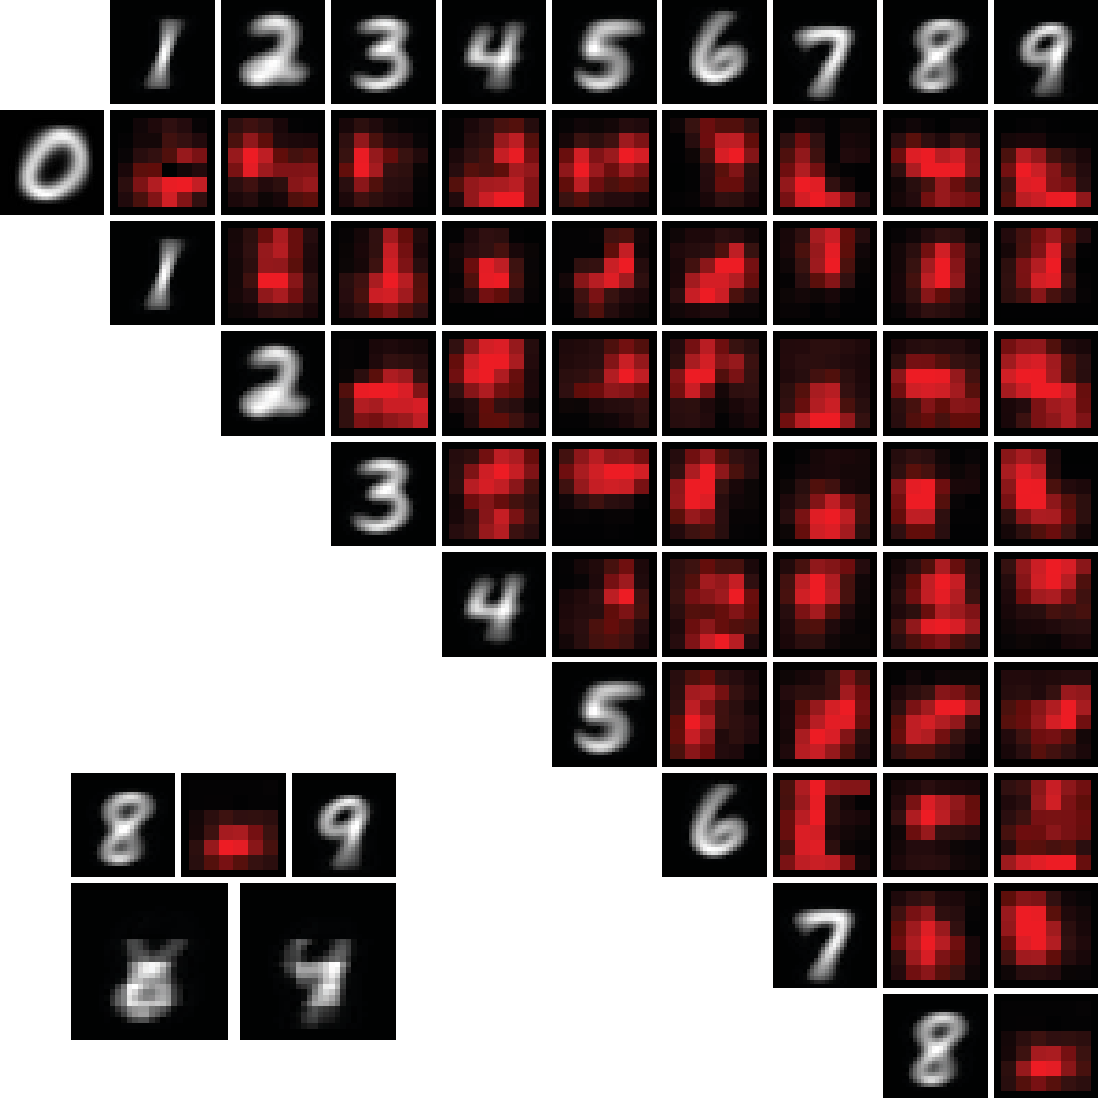
\includegraphics[width=1.\linewidth]{figs/smartpooling/saliency_mnist}
    \end{minipage}
  \caption{Left: Performance comparison (error rate in percentage) on MNIST. Top box: comparison between algorithms using similar pipelines. Bottom box: performance of other related algorithms in the literature. Right: 1-vs-1 saliency maps learned on MNIST. The left-bottom corner plots the mean of digit 8 and 9 multiplied by the corresponding saliency map, showing that the classifier focuses on the bottom part which intuitively also distinguishes the two digits best.}\label{fig:mnist}
\end{figure}

\begin{table}
  \centering
  \begin{tabular}{c|c|c|c}
    \hline
    Method & Codebook & Pooling & Performance\\
    \hline
    ScSPM \cite{Yang:2009vb} & 1024 (SC) & SPM & 73.2$\pm$0.54\\
    LCC+SPM \cite{wang2010locality} & 1024 & SPM & 73.44\\
    \bfseries{Our Method} & 1024 (SC) & OC & {\bfseries 75.3$\pm$0.70}\\
    Boureau et al. \cite{Boureau:2011tz} & 64K & SPM & 77.1$\pm$0.7\\
    \hline
  \end{tabular}
  \begin{tabular}{c|c}
    \hline
    SPM \cite{lazebnik2006beyond} & 64.6$\pm$0.7\\
    NBNN \cite{boiman2008defense} & 72.8$\pm$0.39 (15 training)\\
    Jarret et al. \cite{jarrett2009best} & 65.6$\pm$1.0\\
    RLDA \cite{Karayev2011RLDA} & 73.7$\pm$0.8\\
    Adaptive Deconv. Net \cite{zeileradaptive} & 71.0$\pm$1.0\\
    Feng et al. \cite{Feng:2011wv} & 82.6 \\
    \hline
  \end{tabular}
  \caption{Performance comparison (accuracy in percentage) on Caltech-101. Top: comparison between algorithms using similar pipelines. Bottom: performance of other related algorithms in the literature.}
  \label{tab:caltech}
\end{table}

\subsection{Results on Caltech-101}
Lastly, we report the performance of our algorithm compared with SPM on the Caltech-101 dataset in Table \ref{tab:caltech}. State-of-the-art performance following similar pipelines are also included in the table. Specifically, we used the same two-step pipeline as proposed by Yang et al. \cite{Yang:2009vb}: SIFT features are extracted from 16$\times$16 patches with a stride of 8, and are coded using sparse coding with a codebook of size 1024. For SPM, the coded features are pooled over a pyramid of $1\times1, 2\times2,4\times4$ regular grids; for a fair comparison we also use the $4\times4$ regular grid as our base regions, and select the same number of features as SPM uses.

As can be observed in the table, our pooling algorithm outperforms spatial pooling, although a gap still exists between our result and state-of-the-art methods, which uses more complex coding schemes than that we used. The results suggest that coding is a more dominant factor for the performance of Caltech-101. Existing research, especially the Naive Bayes nearest neighbor method \cite{boiman2008defense}, has also shown a consistent increase of accuracy with higher-dimensional coding output \cite{Boureau:2011tz,yang2010efficient}.
%\footnote{The recent work by Boureau et al. \cite{Boureau:2011tz} could be viewed from the coding perspective by mapping each patch onto the Cartesian space defined by two coding algorithms, and then doing normal spatial pooling to obtain the final global feature.}
However, we still obtain a consistent gain by adopting more flexible receptive fields for pooling, which justifies the effectiveness of the proposed algorithm. Note that the best performance reported by Feng et al. \cite{Feng:2011wv} was obtained by jointly learning the pooling operator ($p$ in $p$-norm pooling) and a per-code spatial saliency map in addition to a larger dictionary, which also follows the idea of learning better spatial information beyond SPM.


\subsection{Transferring Class-Independent Pooling Knowledge}
Beyond classifying existing labels during training, we are also interested in examining whether the learned receptive fields work equally well on unseen classes. While several papers have suggested that simplex cells in V1 performs sparse encoding independent from class labels, and that unsupervised feature learning performs well for the coding step, little is known about the pooling strategy. Learning class-independent pooling knowledge is closely connected to the visual attention model \cite{Itti:2001wa}, which answers the question ``what does an object look like in general''.

To examine the performance of our method against new classes, we utilize the CIFAR-100 dataset, which contains 100 categories with 500 training examples per class. We extract features in the same fashion, and train the SVM classifier with learned codes and receptive fields from CIFAR-10. The classification result is compared against the accuracy rate obtained from directly learning the receptive fields on CIFAR-100, and a baseline that does random feature selection from the same set of overcomplete features. For a fair comparison, all methods use a codebook size of 1,600 and select 6,400 dimensional features. We also tested learning pooled features on CIFAR-100 and testing on CIFAR-10, and the performances are reported in Table \ref{table:transfer}.

\begin{table}
  \centering
  \begin{tabular}{c|l|l}
    \hline
    Classification on & Feature Selection on & Accuracy \\
    \hline
          & CIFAR-10     & {\bfseries 54.88} \\ % training 89.14, reg 0.01
          & CIFAR-100      & 54.83\\ % training 92.39, reg 0.01
    CIFAR-100 %& 2x2 Max Pooling  & 47.26\\ % training 99.62, reg 0.01
          %& 2x2 Ave Pooling  & 47.01\\ % training 78.59, reg 0.001 
          & Random Selection & 54.48$\pm$0.25\\
    \hline
             & CIFAR-100    & 78.88 \\ % training 90.57, reg 0.01
             & CIFAR-10     & {\bfseries 80.17}\\ % reg 0.01
    CIFAR-10 %& 2x2 Max Pooling   & 75.28 \\ % training 86.07, reg 0.01
             %& 2x2 Ave Pooling   & 75.86 \\ % training 90.25, reg 0.0001
             & Random Selection & 78.95$\pm$0.20\\

    \hline
  \end{tabular}
  \caption{The performance of transferring pooled feature between CIFAR-10 and CIFAR-100 compared against natively learned features and random selection.}\label{table:transfer}
\end{table}

The result we obtained showed a mixed message. While the features are leaned from CIFAR-10, they perform well on the CIFAR-100 dataset, and the performance is even better than natively learned features. For the other direction, transferring learned features does not show a statistically significant difference compared with random selection. A possible explanation of such scenario may be that with less training data per class on CIFAR-100, the feature selection algorithm may suffer more from overfitting than it does on CIFAR-10, reducing the generalization ability of the learned features.

In general, our experiment does show the hope for a better and class-independent pooling strategy. Possible future work may involve utilizing larger-scale image databases, and exploring pooled feature learning in an unsupervised approach, which may further reveal valuable pooling strategies.

\section{Summary}

This chapter focused on analyzing the basic coding and pooling component of the state-of-the-art image feature extraction pipelines. Specifically, we show that smarter algorithms that explicitly take into consideration the pooling stage, whether to find better spatial receptive fields or to find pooling-aware lower level dictionaries, provide significant performance boosts in the final classification accuracies.

\section*{Notes}

Parts of this chapter have appeared in peer-reviewed publications as we list below:
\begin{enumerate}
\item Yangqing Jia, Chang Huang, Trevor Darrell. Beyond Spatial Pyramids: Receptive Field Learning for Pooled Image Features. CVPR 2012.
\end{enumerate}